\section{Lecture 12: Square Wells}

\subsection{Infinite Square Well}
We have been considering scattering states in potentials. Now let us consider some kind of bound state
in the Infinite Square Well:
\begin{align*}
    \Psi(x) = \begin{cases}
        0 & \abs*{x} >a \\
        +\infty & \text{otherwise}
    \end{cases}
\end{align*}

We can only match the boundary conditions for $\Psi$ at $x = \pm a$;
we cannot match $\Psi'$. This can only happen at certain energies:

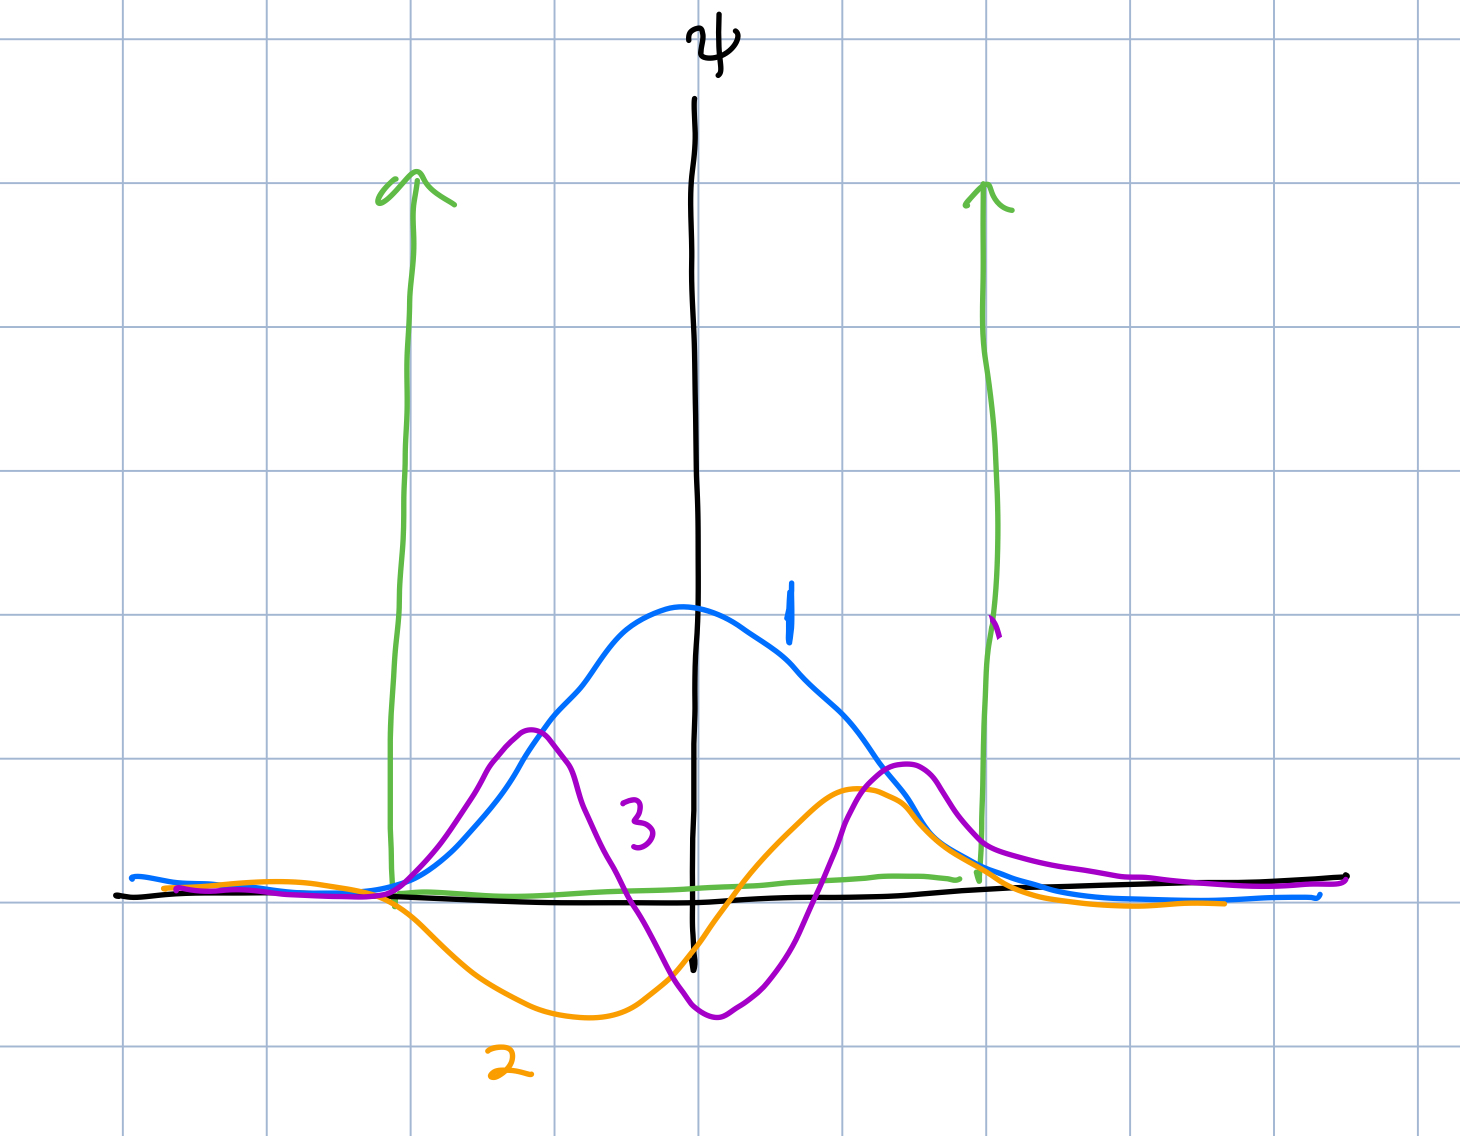
\includegraphics[width=300px]{quantinf.jpeg}

For $|x| < a$, the general solution for a free particle is the superposition of
plane waves with $k = \qty(\frac{2mE}{\hbar^2})^{1/2}$
\[ \Psi(x) = Ae^{ikx} + Be^{-ikx}  = A \cos(kx) + B \sin(kx) \]
\begin{theorem}
With a potential with even symmetry, there are only even and odd solutions for $\Psi$.
\end{theorem}

The boundary conditions end up being:
\begin{align*}
    A \cos(ka) + B \sin(ka) &= 0 \\
    A \cos(ka) - B \sin(ka) &= 0 \\
\end{align*}
which means: $A \cos(ka) = B \sin(ka) = 0$

Suppose $B = 0$ for even solutions. Then: $\cos(ka) = 0$, so $k_n = \frac{n\pi}{2a} = \frac{n\pi}{L}$ for $n = 1, 3, \dots$
and our solution is $\Psi_n(x) = A_n \cos(k_n x)$ and:
\begin{align*}
    \int \Psi_n^* \Psi_n \dd{x} &= 1 \implies A = \frac{1}{\sqrt{a}}
\end{align*}
So the general solution is:
\[ \Psi_n(x) = \frac{1}{\sqrt{a}} \cos(\frac{n\pi x}{2a}) \]

Similarly for $A = 0$, we can quantize for $n = 2, 4, 6, \dots$.
\[ \Psi_n(x) = \frac{1}{\sqrt{a}} \sin\qty(\frac{n\pi x}{2a}) \]

For all $n \in \N$, $k_n = \frac{n\pi}{L}$. Whenever you can fit a half-wavelength between the boundaries, you get a bound state.
\[ E_n = \frac{p^2}{2m} = \frac{\hbar^2 k_n^2}{2m} = \frac{k^2 \pi^2 n^2}{2mL^2} \]

This is a decent approximation to an atom for low $n$ states. There are an infinite number of bound states, though, which is
unrealistic. The ground state energy $E_1$ is not 0. $E_n \propto n^2$.

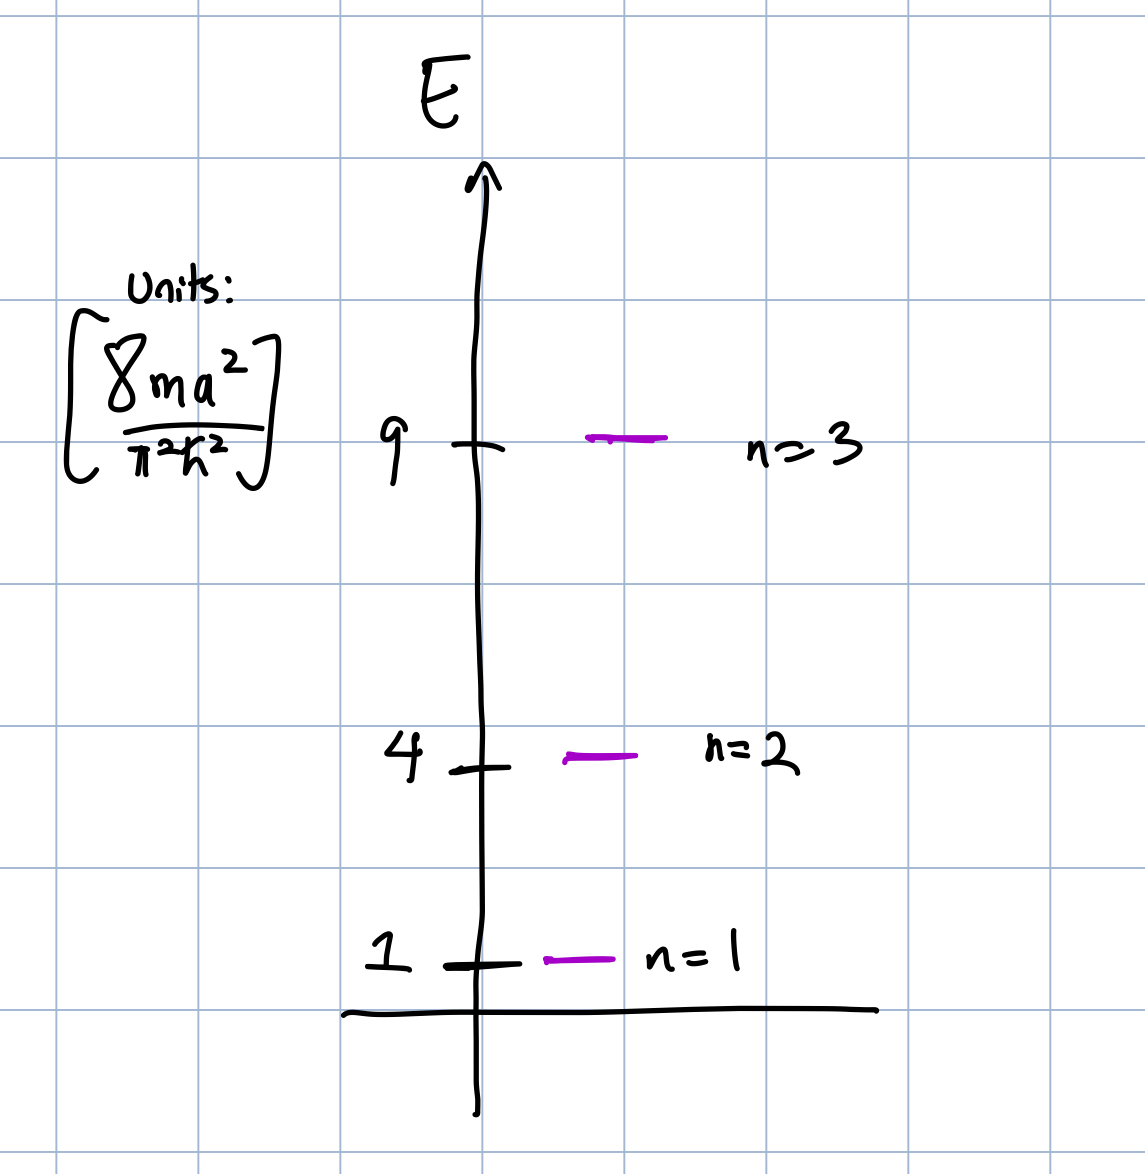
\includegraphics[width=250px]{infnrg.jpeg}

\subsection{Finite Square Well}
Now consider a finite version of the above.

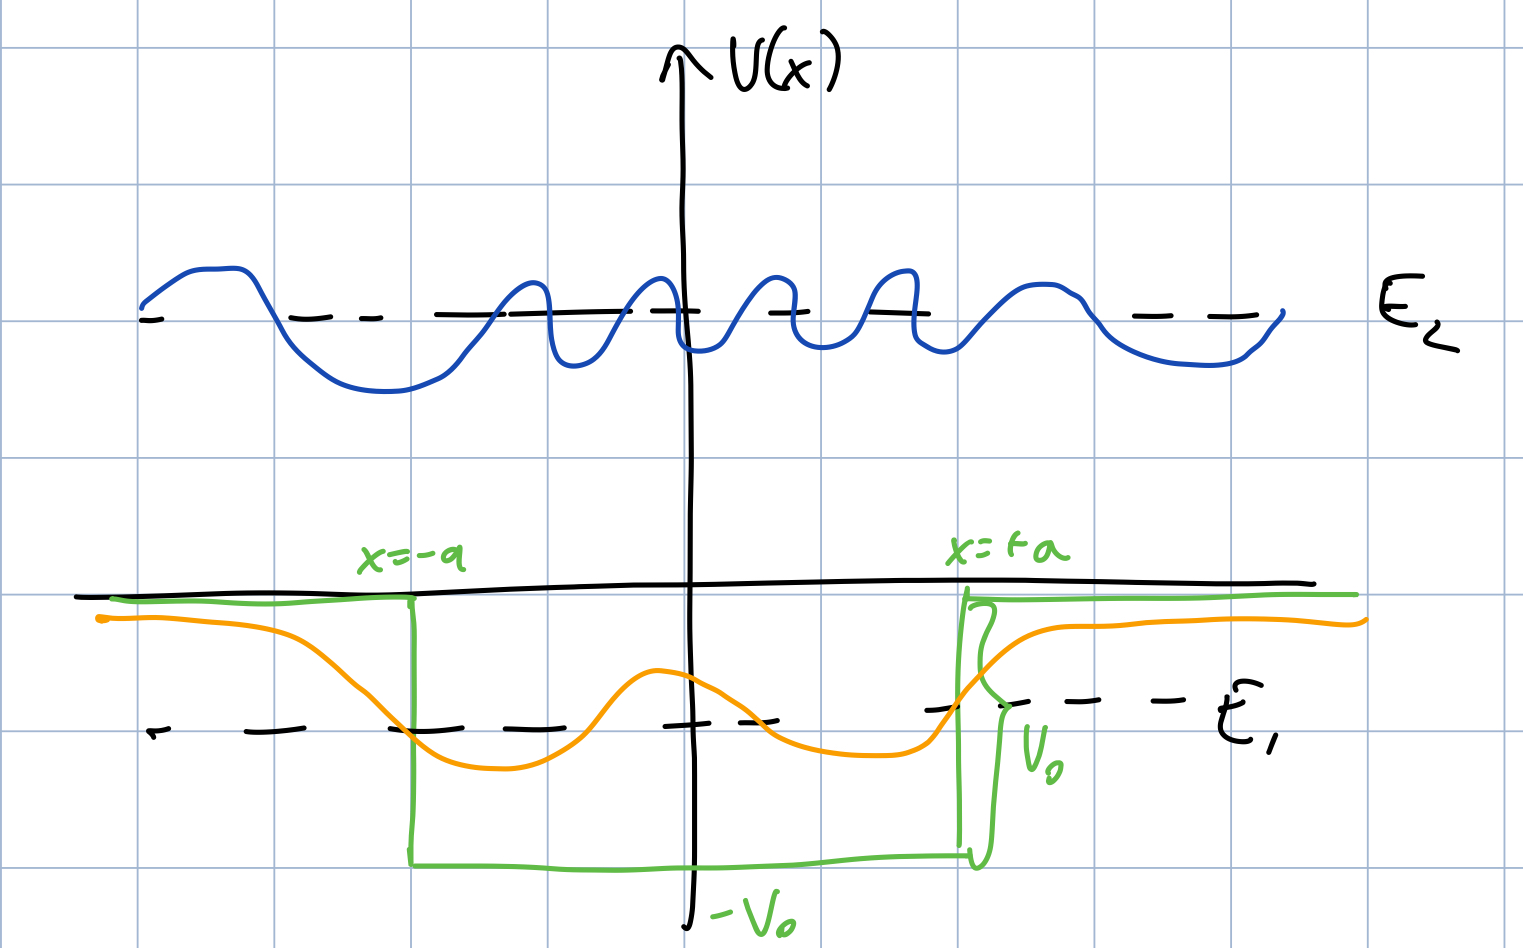
\includegraphics[width=300px]{finwell.jpeg}

Consider case 1, $-V_0 < E < 0$.
Take $\alpha = \qty[\frac{2m}{\hbar^2}(V_0 + E)]^{1/2} = \qty[\frac{2m}{\hbar^2}(V_0 - |E|)]^{1/2}$.
Then we know
\[ \derivative{^2 \Psi(x)}{x^2} +\alpha^2 \Psi(x) = 0 \]
inside the well.

Now suppose you are outside the well:
you have $\beta = (\frac{2m|E|}{\hbar^2})^{1/2}$.
\[ \derivative{^2 \Psi(x)}{x^2} - \beta^2 \Psi(x) = 0 \]
So the even solutions look like:
\[
    \Psi(x) = \begin{cases}
        A \cos(\alpha x) & |x| < a \\
        Ce^{-\beta x} & |x| > a
    \end{cases}\]

Matching boundary conditions:
\begin{align*}
    \Psi: A \cos(\alpha a) = Ce^{-\beta a} \\
    \Psi': - \alpha A \sin(\alpha a) = -\beta Ce^{-\beta a} \\
    \alpha \tan(\alpha a) = \beta C e^{-\beta a}
\end{align*}

For the odd solutions:
\[ \Psi(x) = \begin{cases}
    B \sin(\alpha x) & |x| < a\\
    Ce^{-\beta x} & |x| > a
\end{cases}\]

Now matching boundary conditions yields $\alpha \cot(\alpha a) = -\beta$.
Solving these two transcendental equations is kinda tricky. Define $\xi = \alpha a$,
$\eta = \beta a$, meaning that:
\begin{align*}
    \xi \tan \xi &= \eta \\
    \xi \cot \xi &= - \eta
\end{align*}
Note that $\xi^2 + \eta^2 = \delta^2$ where $\delta = \qty(\frac{2mV_0 a^2}{\hbar^2})^{1/2}$.
The solutions are the intersections here:

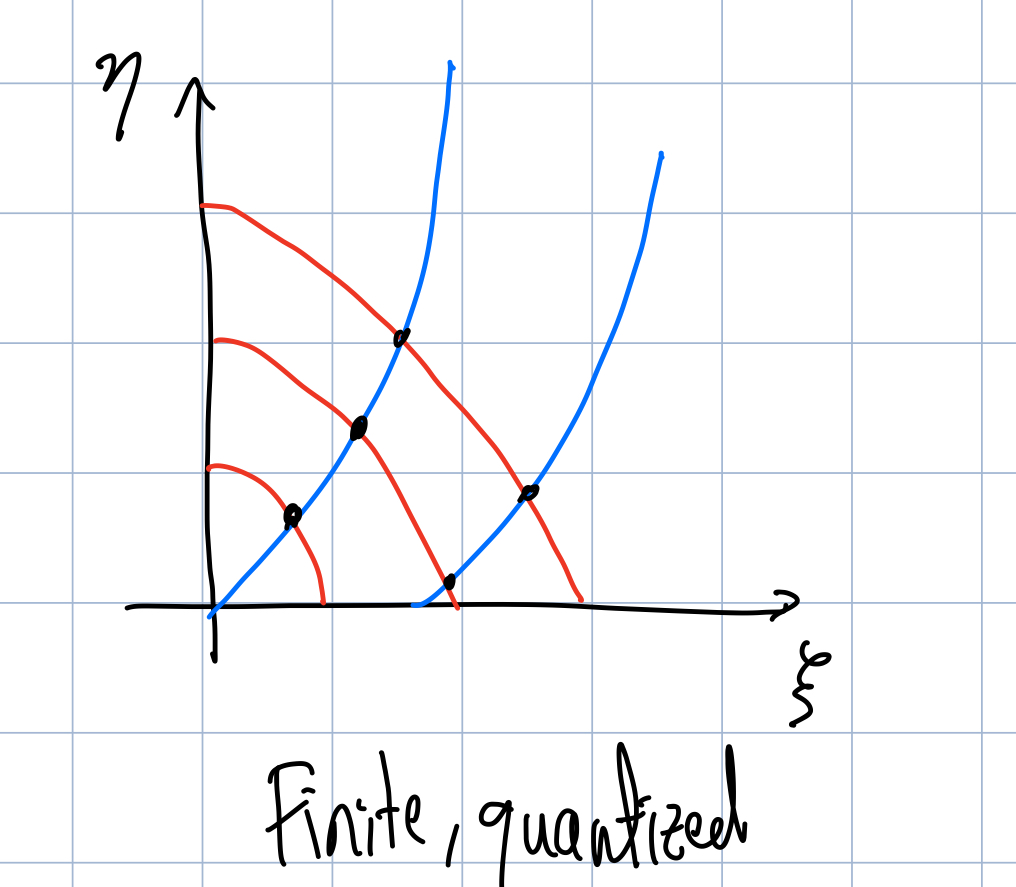
\includegraphics[width=200px]{xiquant.jpeg}

which are a finite number of quantized bound states. The spectrum
and wave function look like this:

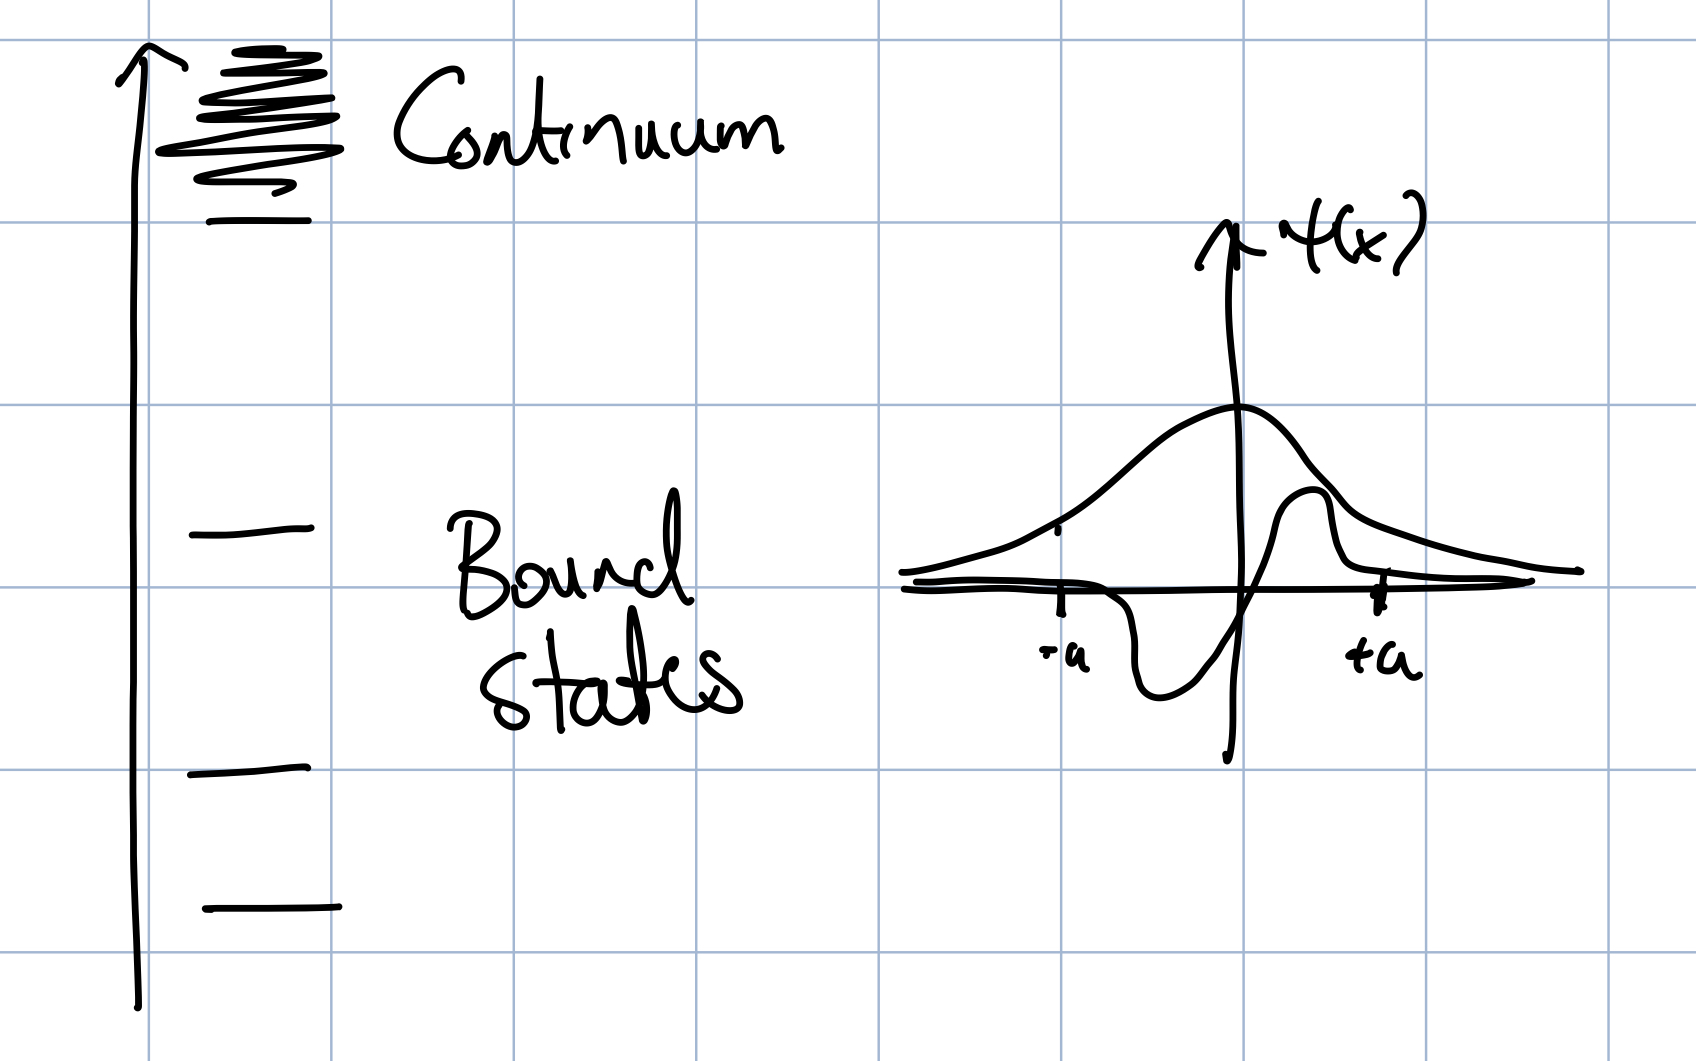
\includegraphics[width=300px]{why_not_both.jpeg}

which seems like a much better approximation of an atom (since you can ``pull off" electrons
and have non-bound states).

Finally, case 2 is really easy, it's the same traveling wave.

\[
    \Psi(x) = \begin{cases}
        Ae^{ikx} + Be^{-ikx} & x < -a \\
        Ce^{ikx} & x > a \\
        Fe^{i \alpha x} + Ge^{-i\alpha x} & |x| < a
    \end{cases} \]

where $k$ and $\alpha$ are found the same way as always.

\[ \mathfrak{R} = \qty[1 + \frac{4E(V_0 + E)}{V_0^2 \sin^2(\alpha L)}]^{-1} \]
etc.